\begin{figure*}
  \centering
  \begin{subfigure}[b]{0.5\textwidth}
    \centering
    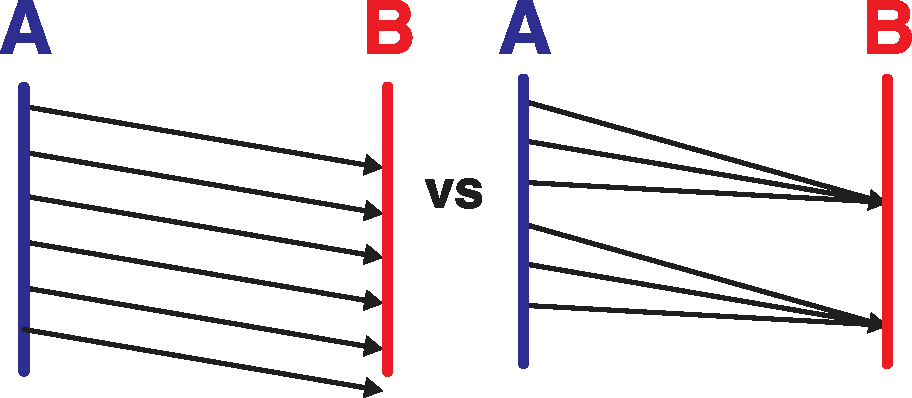
\includegraphics[width=\linewidth]{img/quality-of-service-metric-definitions/clumpiness.pdf}
    \caption{Bunching}
    \label{fig:quality-of-service-metric-definitions-clumpiness}
  \end{subfigure}%
  \begin{subfigure}[b]{0.5\textwidth}
    \centering
    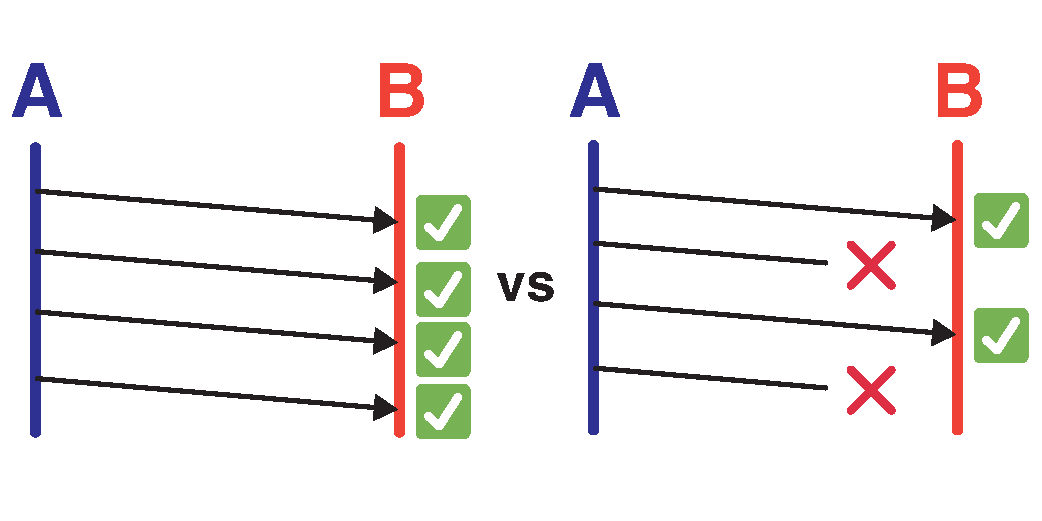
\includegraphics[width=\linewidth]{img/quality-of-service-metric-definitions/delivery-failure-rate.pdf}
    \caption{Delivery Failure Rate}
    \label{fig:quality-of-service-metric-definitions-delivery-failure-rate}
  \end{subfigure}
  \begin{subfigure}[b]{0.5\textwidth}
    \centering
    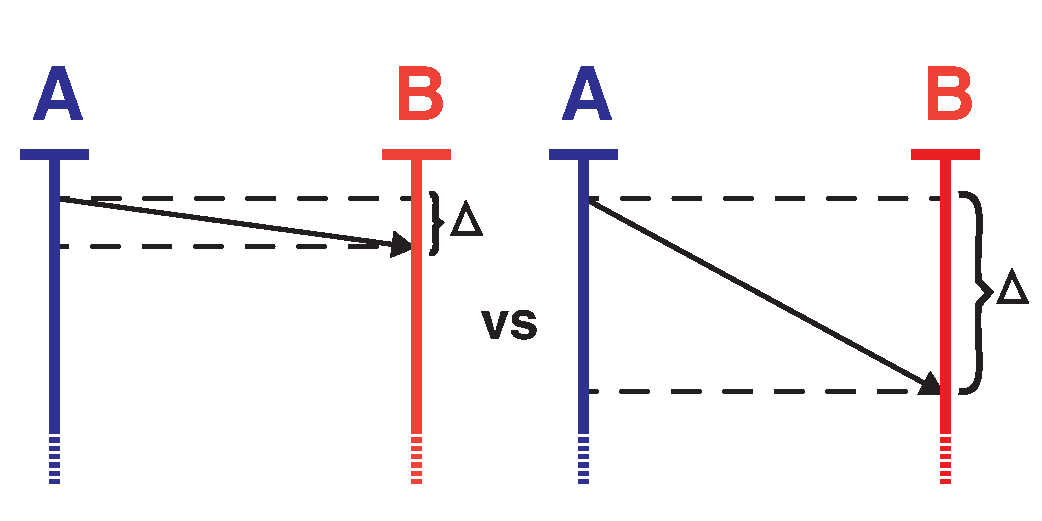
\includegraphics[width=\linewidth]{img/quality-of-service-metric-definitions/latency.pdf}
    \caption{Latency}
    \label{fig:quality-of-service-metric-definitions-latency}
  \end{subfigure}%
  \begin{subfigure}[b]{0.5\textwidth}
    \centering
    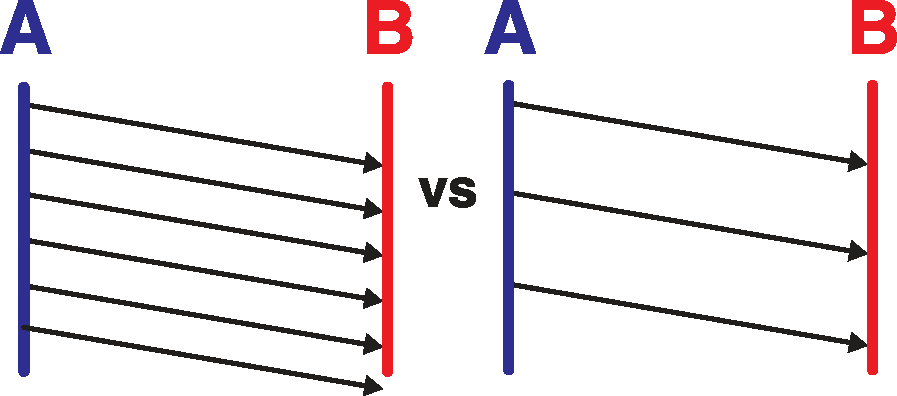
\includegraphics[width=\linewidth]{img/quality-of-service-metric-definitions/simstep-period.pdf}
    \caption{Update Period}
    \label{fig:quality-of-service-metric-definitions-simstep-period}
  \end{subfigure}%
  \caption{
  Quality of service metrics.
  Each illustration is a space-time diagram, with $A$ and $B$ representing independent processes.
  The vertical axis depicts the passage of time, from top to bottom.
  Solid black arrows represent message delivery.
  The left panel of each metric's diagram depicts a scenario with a lower (``better'') value for that metric compared to the right panel, which depicts a higher (``worse'') value for that metric.
  }
  \label{fig:quality-of-service-metric-definitions}
\end{figure*}
